Een spoel\index{Spoel}\index{Coil} is een stuk geleider die opgerold is tot een rolletje.

Als we een spanning zetten op deze spoel van vormt hij een magnetisch veld. Er ontstaat dus een noord-pool en een zuid-pool en hij werkt dan als een, zwakke, magneet.

In de elektronica wordt een switch weergegeven met het symbool dat je ziet weergegeven in \ref{symbool:spoel}

\begin{figure}[h]
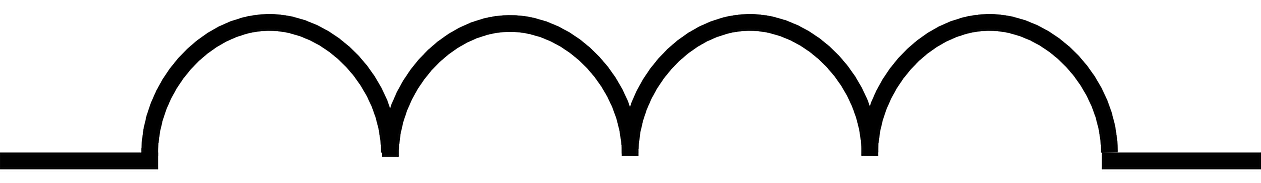
\includegraphics[width=5cm]{spoel}
\centering
\caption{Symbool van een spoel}
\label{symbool:spoel}
\end{figure}

Zetten we een wisselspanning op de spoel dan zullen de noord- en zuidpool wisselen van de ene kant van de spoel naar de andere.

